\documentclass[conference]{IEEEtran}
\usepackage{amsmath,amssymb,amsfonts}
\usepackage{xcolor}
\usepackage{tikz}
\usetikzlibrary{arrows,fit,positioning}
\usetikzlibrary{shapes.geometric}
\usepackage{pgfplots}
\pgfplotsset{width=11cm,compat=1.9}

\begin{document}

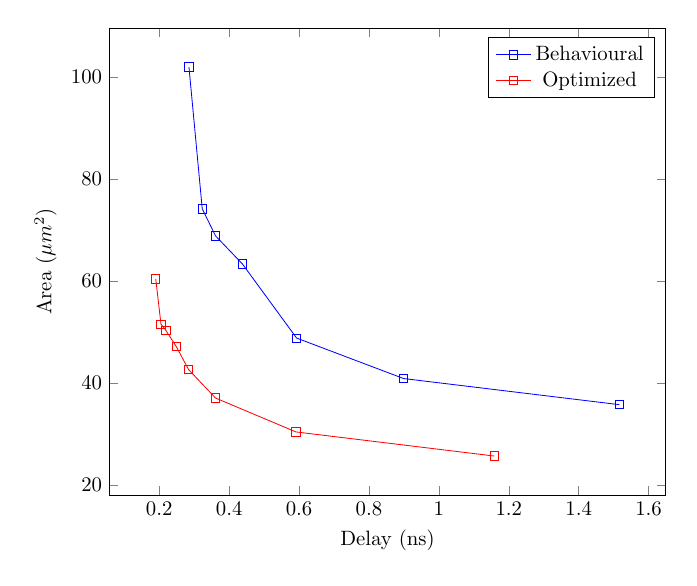
\begin{tikzpicture}[scale=0.75]
\begin{axis}[
    xlabel ={Delay (ns)},
    ylabel ={Area ($\mu m^2$)}
    ]
\addplot[
    color=blue,
    mark=square,
    ]
    coordinates {
        (0.285, 101.99808)
        (0.323, 74.20032 )
        (0.361, 68.89248 )
        (0.438, 63.37944 )
        (0.593, 48.85128 )
        (0.899, 40.91688 )
        (1.516, 35.80056 )
        % (2.748, 31.86072 )
    };
    \addlegendentry{Behavioural}
    \addplot[
    color=red,
    mark=square,
    ]
    coordinates {
        (0.19 , 60.45192)
        (0.205, 51.5736 )
        (0.219, 50.35608)
        (0.249, 47.15496)
        (0.284, 42.66792)
        (0.361, 37.10016)
        (0.591, 30.45168)
        (1.159, 25.7184 )
    };
    \addlegendentry{Optimized}
\end{axis}
\end{tikzpicture}

\end{document}